% !TEX TS-program = XeLaTeX
% use the following command: 
% all document files must be coded in UTF-8
\documentclass{textolivre}
% for anonymous submission
%\documentclass[anonymous]{textolivre}
% to create HTML use 
%\documentclass{textolivre-html}
% HTML compile using make4ht
% $ make4ht -c textolivre-html.cfg -u -x article "fn-in,svg,pic-align"   
%
% See more information on the repository: https://github.com/leolca/textolivre

% Metadata
\begin{filecontents*}[overwrite]{article.xmpdata}
    \Title{Narrativas de evolução: uma análise da tecnobiografia de uma professora de inglês}
    \Author{Mauricio Teixeira Mendes}
    \Language{pt-BR}
    \Keywords{Análise narrativa \sep Tecnologias digitais \sep Letramento \sep Evolução}
    \Journaltitle{Texto Livre}
    \Journalnumber{1983-3652}
    \Volume{14}
    \Issue{1}
    \Firstpage{1}
    \Lastpage{16}
    \Doi{10.35699/1983-3652.2021.26711}

    \setRGBcolorprofile{sRGB_IEC61966-2-1_black_scaled.icc}
            {sRGB_IEC61966-2-1_black_scaled}
            {sRGB IEC61966 v2.1 with black scaling}
            {http://www.color.org}
\end{filecontents*}

% used to create dummy text for the template file
\definecolor{dark-gray}{gray}{0.35} % color used to display dummy texts
\usepackage{lipsum}
\SetLipsumParListSurrounders{\colorlet{oldcolor}{.}\color{dark-gray}}{\color{oldcolor}}

% used here only to provide the XeLaTeX and BibTeX logos
\usepackage{hologo}

% used in this example to provide source code environment
%\crefname{lstlisting}{lista}{listas}
%\Crefname{lstlisting}{Lista}{Listas}
%\usepackage{listings}
%\renewcommand\lstlistingname{Lista}
%\lstset{language=bash,
        breaklines=true,
        basicstyle=\linespread{1}\small\ttfamily,
        numbers=none,xleftmargin=0.5cm,
        frame=none,
        framexleftmargin=0.5em,
        framexrightmargin=0.5em,
        showstringspaces=false,
        upquote=true,
        commentstyle=\color{gray},
        literate=%
           {á}{{\'a}}1 {é}{{\'e}}1 {í}{{\'i}}1 {ó}{{\'o}}1 {ú}{{\'u}}1 
           {à}{{\`a}}1 {è}{{\`e}}1 {ì}{{\`i}}1 {ò}{{\`o}}1 {ù}{{\`u}}1
           {ã}{{\~a}}1 {ẽ}{{\~e}}1 {ĩ}{{\~i}}1 {õ}{{\~o}}1 {ũ}{{\~u}}1
           {â}{{\^a}}1 {ê}{{\^e}}1 {î}{{\^i}}1 {ô}{{\^o}}1 {û}{{\^u}}1
           {ä}{{\"a}}1 {ë}{{\"e}}1 {ï}{{\"i}}1 {ö}{{\"o}}1 {ü}{{\"u}}1
           {Á}{{\'A}}1 {É}{{\'E}}1 {Í}{{\'I}}1 {Ó}{{\'O}}1 {Ú}{{\'U}}1
           {À}{{\`A}}1 {È}{{\`E}}1 {Ì}{{\`I}}1 {Ò}{{\`O}}1 {Ù}{{\`U}}1
           {Ã}{{\~A}}1 {Ẽ}{{\~E}}1 {Ũ}{{\~u}}1 {Õ}{{\~O}}1 {Ũ}{{\~U}}1
           {Â}{{\^A}}1 {Ê}{{\^E}}1 {Î}{{\^I}}1 {Ô}{{\^O}}1 {Û}{{\^U}}1
           {Ä}{{\"A}}1 {Ë}{{\"E}}1 {Ï}{{\"I}}1 {Ö}{{\"O}}1 {Ü}{{\"U}}1
           {ç}{{\c{c}}}1 {Ç}{{\c{C}}}1
}


\journalname{Texto Livre: Linguagem e Tecnologia}
\thevolume{14}
\thenumber{1}
\theyear{2021}
\receiveddate{\DTMdisplaydate{2020}{05}{31}{-1}} % YYYY MM DD
\accepteddate{\DTMdisplaydate{2020}{8}{11}{-1}}
\publisheddate{\DTMdisplaydate{2020}{12}{22}{-1}}
% Corresponding author
\corrauthor{Mauricio Teixeira Mendes}
% DOI
\articledoi{10.35699/1983-3652.2021.26711}
% list of available sesscions in the journal: articles, dossier, reports, essays, reviews, interviews, editorial
\articlesessionname{Linguística e Tecnologia}
% Abbreviated author list for the running footer
\runningauthor{Mendes}
\editorname{Daniervelin Pereira}

\title{Narrativas de evolução: uma análise da tecnobiografia de uma professora de inglês}
\othertitle{Narratives of evolution: an analysis of the technobiography of an english teacher}
% if there is a third language title, add here:
%\othertitle{Artikelvorlage zur Einreichung beim Texto Livre Journal}

\author[1]{Mauricio Teixeira Mendes \orcid{0000-0001-9619-5903} \thanks{Email: \url{mauricioedocampo@gmail.com}}}

\affil[1]{Universidade Federal de Minas Gerais, Belo Horizonte, MG, Brasil.}

\addbibresource{article.bib}
% use biber instead of bibtex
% $ biber tl-article-template

% set language of the article
\setdefaultlanguage[variant=brazilian]{portuguese}
\setotherlanguage{english}

% for spanish, use:
%\setdefaultlanguage{spanish}
%\gappto\captionsspanish{\renewcommand{\tablename}{Tabla}} % use 'Tabla' instead of 'Cuadro'

% for languages that use special fonts, you must provide the typeface that will be used
% \setotherlanguage{arabic}
% \newfontfamily\arabicfont[Script=Arabic]{Amiri}
% \newfontfamily\arabicfontsf[Script=Arabic]{Amiri}
% \newfontfamily\arabicfonttt[Script=Arabic]{Amiri}
%
% in the article, to add arabic text use: \textlang{arabic}{ ... }

\usepackage{xcolor,colortbl}

\begin{document}
\maketitle

\begin{polyabstract}
\begin{portuguese}
\begin{abstract}
O presente trabalho é uma análise de narrativa, em que é explanado brevemente o conceito de pesquisa narrativa, e algumas questões pontuais encontradas durante a leitura e análise de uma narrativa de aprendizagem de tecnologia digital de uma pós-graduanda dessa instituição. Nessas análises são observados alguns pontos como: metáforas, marcos históricos, pequenas histórias e outras observações. Além disso, na conclusão é feita uma comparação da narrativa analisada com a trajetória de vida do autor deste texto.

\keywords{Análise narrativa \sep Tecnologias digitais \sep Letramento \sep Evolução}
\end{abstract}
\end{portuguese}

\begin{english}
\begin{abstract}
The present study is a narrative analysis, where the concept of narrative research is briefly explained, as well as some specific questions encountered during the reading and analysis of a digital technology learning narrative of a graduate student from this institution. Some points explored in the analysis are: metaphors, historical landmarks, small histories and other observations. In addition, in the conclusion a comparison of the analyzed narrative with the life trajectory of the author of this text is made.

\keywords{Narrative analysis \sep Digital technologies \sep Literacy \sep Evolution}
\end{abstract}
\end{english}

% if there is another abstract, insert it here using the same scheme
\end{polyabstract}


\section{Introdução}\label{sec-intro}
Este artigo reporta a análise de uma narrativa de uma professora de inglês, discente do Programa de Pós-Graduação em Estudos Linguísticos da Faculdade de Letras (FALE) da Universidade Federal de Minas Gerais (UFMG). Tanto a mestranda como o autor deste texto estavam matriculados na disciplina “Pesquisa Narrativa”, cujo trabalho final demandava a análise de uma narrativa de aprendizagem de qualquer língua, ou sobre o processo de aprendizagem de tecnologia digital. Os professores da disciplina, Vera Menezes e Ronaldo Gomes Jr., fizeram um cronograma direcionando os discentes sobre qual narrativa deveriam analisar. De acordo com o cronograma, dever-se-ia analisar a narrativa de aprendizagem de tecnologia digital de uma estudante. Para preservar a identidade da autora da autobiografia analisada, optou-se o uso do pseudônimo Clarice.

No decorrer do texto, apresentaremos algumas questões teóricas sobre pesquisa narrativa e tecnobiografia, que seria, segundo \textcite{kennedy2003}, uma narrativa biográfica sobre as relações e trajetória do sujeito com as tecnologias. Analisaremos e discutiremos dados que foram extraídos da narrativa em questão, como narrativas de evolução, narrativas dicotômicas, metáforas e pequenas histórias.

\section{Narrativas e Tecnobiografias}\label{sec-narrativas}
Nesta seção apresentaremos alguns conceitos sobre a pesquisa narrativa, bem como discorreremos sobre o seu papel investigativo no processo de ensino e aprendizagem. Como este artigo trata de uma análise de uma tecnobiografia, também abordaremos esse conceito. 

Ao longo da história, a narrativa, seja oral ou escrita, circula na sociedade por meio de histórias (re)contadas, relatos de eventos reais ou fictícios, dentre outros. Segundo \textcite[p.~3]{riessman1993}, a arte de contar histórias de eventos passados é uma “atividade humana universal”. A narrativa como objeto de estudo, a pesquisa narrativa, surge no início do século XX no campo da Psicologia, quando biografias eram utilizadas para investigação de indivíduo e suas condições sociais. Em meados do século XX, as ciências sociais começam, então, a explorar a pesquisa narrativa no cenário do ensino e aprendizagem de línguas.

Para \textcite[p.~7, tradução nossa]{barkuizen2014}, as narrativas “são textos falados ou escritos, são produzidos por pessoas que têm algo a dizer, estão situados no tempo e no espaço, (\ldots), tem propósito e significado dentro do contexto de sua narração”\footnote{“are spoken or written texts, are produced by people who have something to tell, are situated in time and space, (\ldots), have purpose and meaning within the context of their telling”.}.

De acordo com \textcite{barkuizen2014}, Jerome Bruner, um dos pioneiros na pesquisa narrativa, descreve duas maneiras básicas de pensamentos, a saber: “história” e “argumento”, que mais tarde são chamados de “paradigmáticos” e “narrativos”. Nessa classificação, “os argumentos convencem de sua ‘verdade’, apelando aos procedimentos para estabelecer provas formais e empíricas; as histórias convencem de sua ‘vitalidade’, apelando mais aos critérios de verossimilhança \cite[p.~1, tradução nossa]{barkuizen2014}”\footnote{“Arguments convince of their ‘truth’, appealing to procedures for establishing formal and empirical proof; stories convince of their ‘lifelikeness’, appealing more to criteria of verisimilitude”.}. O pensamento paradigmático se associa também ao desenvolvimento do pensamento racional, porém “pode levar a conclusões divorciadas da realidade vivida dos fenômenos (\ldots), justamente porque lhes falta a qualidade de vida que esperamos de uma boa história” \cite[p.~1, tradução nossa]{barkuizen2014}\footnote{“can lead to conclusions that are divorced from the lived reality of phenomena (\ldots), precisely because they lack the quality of lifelikeness that we expect of a good story”.}.

Partindo das críticas ao pensamento paradigmático, surge uma “virada narrativa”, na qual a pesquisa narrativa torna-se um modo legítimo de pensar e escrever. Emerge uma variedade de abordagens complementares, experimentação, observação, pesquisa, entre outros métodos, e um paradigma alternativo para pesquisa social, com o foco em como as pessoas usam histórias para dar sentido às suas experiências \cite{barkuizen2014}.

\textcite{clandinin2000} traçam uma linha de conceitos e de pesquisadores na área de pesquisa narrativa, quando percebe-se a ideia de elo entre a narrativa e a vida. Dentre os pesquisadores, destacam-se Dewey, Coles e Polkinghorne. \textcite[p.~12, tradução nossa]{clandinin2000} explicam que, para Dewey, a experiência é pessoal e social e as pessoas são indivíduos que participam de um contexto social e precisam ser entendidas nessa inter-relação. Já Coles parte da psiquiatria para a narrativa e “aprende sobre a vida-morte, casamento, moralidade – de seus pacientes e seus alunos”\footnote{"Coles learns about life-death, marriage, morality- from his patients and his students".}. Os autores ainda mencionam que, de acordo com Polkinghorne, a narrativa é uma pesquisa “ainda em seus estágios iniciais. Por incluir a dimensão temporal em sua estrutura organizacional, é muito diferente da organização formal que coloca ‘fatos’ em categorias” \cite[p.~16]{clandinin2000}\footnote{Polkinghorne believes that narrative research is research "still in its early stages. Because it includes the temporal dimension in its organizational structure, it is very different from the formal organization that puts 'facts' into categories”.}.

Em sua maioria, as pesquisas narrativas na área da Linguística Aplicada se ocupam da análise do ensino e aprendizagem de línguas. Por exemplo, \textcite{barkuizen2014} citam uma pesquisa narrativa de Menezes (2008), que faz uma análise estrutural temática sobre como os alunos construíram aberturas e fechamentos de histórias de aprendizagem de línguas (Language Learning Histories – LLHs):

\begin{quote}
Ela concluiu que o conhecimento da segunda língua não é apenas “um produto de contextos formais de aprendizagem, mas surge da interação de diferentes redes sociais (família, produção cultural, escola) com os fatores cognitivos e afetivos individuais” (p. 213). Essa conclusão é baseada tanto no conteúdo quanto no discurso das narrativas – sobre o que os alunos dizem, mas, mais importante, sobre como eles organizam o que dizem \cite[p.~82, tradução nossa]{menezes2008}\footnote{“She concluded that second language knowledge is not only “a product of formal learning contexts, but it emerges out of the interaction of different social networks (family, cultural production, school) with the individual cognitive and affective factors” \cite[p.~213]{menezes2008}. This conclusion is based on both the content and discourse of the narratives — on what the learners say, but more importantly how they organize what they say”.}.
\end{quote}

Apesar de os contextos da pesquisa narrativa na área da Linguística Aplicada, em sua maioria, como no exemplo acima, pesquisarem o ensino e a aprendizagem de segunda língua ou língua adicional, entende-se que esses processos ocorrem em várias esferas, e a pesquisa narrativa pode contribuir para entender outros contextos, como, por exemplo, a relação o sujeito e as tecnologias digitais, o que vai ao encontro deste artigo, cujo objetivo é a análise de uma tecnobiografia.

De acordo com \textcite{kennedy2003}, tecnobiografia é um tipo de narrativa que relaciona história de vida com tecnologias digitais. Para compreender as relações sujeito-tecnologias, principalmente as digitais, precisamos observar histórias de vidas de indivíduos situados dentro das relações sociais, de consumo e produção de tecnologias de informação e comunicação. Ainda segundo o autor, “(\ldots) histórias vividas, ou tecnobiografias, são significantes por causa das diferenças sutis e nuances em cada experiência individual com a tecnologia” \cite[p.~120, tradução nossa]{kennedy2003}7\footnote{“(\ldots) individual experience stories, or technobiografies, are significant because of the subtle e nuanced differences in each individual’s techno experiences”.}

\section{Metodologia}\label{sec-metodologia}
De acordo com \textcite[p.~72]{barkuizen2014}, a pesquisa narrativa é uma forma de pesquisa qualitativa, e os “estudos narrativos geralmente empregam as mesmas abordagens de análise de dados que são usadas em outros tipos de pesquisa qualitativa”\footnote{“narrative studies often employ the same approaches to data analysis that are used in other types of qualitative research”.}. Assim sendo, por se tratar de uma pesquisa qualitativa de paradigma interpretativista, na análise de dados deste trabalho serão utilizadas análises temáticas, metafóricas, estruturais e outras.

Em cada caso, a escolha da metodologia de análise de dados é justificada pelos objetivos do pesquisador. Para a análise da narrativa em questão, não havia um tema predeterminado. Porém, o próprio gênero, tecnobiografia, é sugestivo a atentar para os processos de aprendizagem com as tecnologias digitais e a relação sujeito-tecnologia. 

Tendo como principal objetivo compreender como foi o processo de aprendizagem de Clarice com as tecnologias digitais, para a análise dos dados foram seguidos os seguintes passos: 
\begin{enumerate*}[label=\itshape\arabic*\upshape)]
\item leitura e releitura de toda a narrativa; 
\item destaque de todos os trechos considerados relevantes para a temática; 
\item agrupamento dos trechos de acordo com regularidades semânticas, criando categorias; e 
\item criação de um quadro com pontos de divergências categorizados como vantagens e desvantagens em relação ao uso das tecnologias digitais.
\end{enumerate*}

Ao citar metodologias de Gao (2010) e Sakui (2002) \textcite{barkuizen2014} chamam a atenção para os riscos que envolve a análise de conteúdo com temas pré-determinados, pois ela pode impedir que se aprofunde em outras análises de dados emergentes. O exercício de (re)leitura, o ir e vir entre os trechos selecionados, leituras bibliográficas e outras pesquisas para entender questões particulares e gerais da personagem, fizeram emergir outras temáticas, como: metáforas, pequenas histórias e a comparação da narrativa analisada com a própria trajetória do autor deste texto.

\section{Análise e discussão dos dados}\label{sec-analise}
Nesta seção, apresentamos e discutimos as categorias que emergiram na análise de dados. Primeiramente, contextualizamos a autora da tecnobiografia. Em um segundo momento, apresentamos e discutimos alguns dados sobre as narrativas de evolução em dois momentos: a evolução de Clarice em relação às tecnologias digitais e aos constantes avanços de tais tecnologias. Na subseção “Narrativas dicotômicas”, trazemos excertos em que a narradora descreve as vantagens e desvantagens das tecnologias digitais. Em seguida, discorremos sobre outra temática que surgiu no decorrer da análise, na subseção “Metáforas”, em que discutimos excertos em que emergem “metáforas ontológicas” \cite{lakoff1980} e “identidades metaforizadas” \cite{gomes2016}. Nas subseções “Pequenas histórias”, analisamos excertos nos quais a narradora, dentro de sua tecnobiografia, “abre parênteses” e apresenta pequenas narrativas de suas relações sociais. Por fim, na subseção “Minha vida é uma narrativa”, estabelecemos uma reação entre a trajetória do autor deste texto com a narrativa da participante.

\subsection{Narrativas de evolução}\label{sec-evolucao}
Clarice nasceu na década de 80 é natural da cidade de Belo Horizonte, Minas Gerais. É filha de um mecânico industrial e de uma professora. Sua infância, adolescência e a passagem pela educação básica foram na cidade de Santa Bárbara, Minas Gerais. Aos 15 anos, Clarice começou a frequentar um curso de inglês, que acabara motivando-a ao interesse pela docência. Assim que ela concluiu o Ensino Médio ingressou em uma licenciatura em Letras, na Universidade Federal de Viçosa, tornando-se, assim, uma professora. Nos dias atuais, ela é mestranda do programa de pós-graduação em Estudos Linguísticos da UFMG e acumula cerca de 15 anos de experiência na docência em escolas públicas, particulares e cursos de idiomas.

Em uma leitura geral da tecnobiografia, pudemos perceber várias narrativas de evolução, nas quais Clarice se representa como um indivíduo que evolui, ao mesmo tempo em que as tecnologias digitais passam por constantes mudanças, que podem ser constatadas nos excertos abaixo (\Cref{fig01}): 

\begin{figure}[htbp]
 \centering
 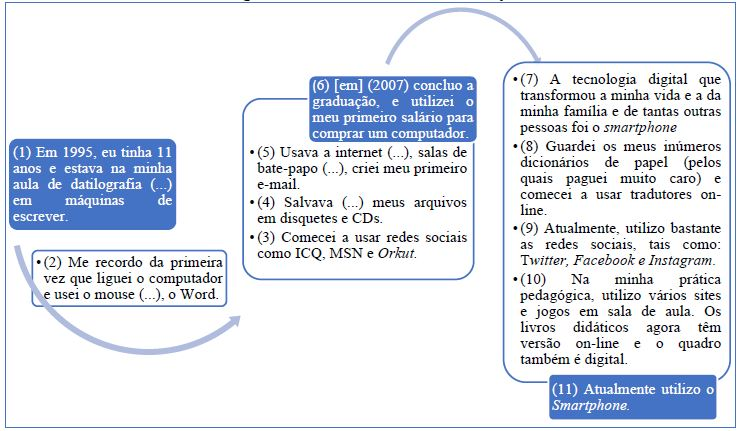
\includegraphics[width=0.85\textwidth]{fig01.png}
 \caption{Narrativas de evolução.}
 \label{fig01}
 \source{Elaborado pelo autor.}
\end{figure}

Os excertos apresentados no quadro acima seguem a estrutura narrativa da tecnobiografia de Clarice, na qual relata sua primeira experiência com as tecnologias digitais no ano de 1995 (excerto 1), perfaz um caminho de conquista e aprendizagem com as tecnologias digitais (excerto 6) e finaliza falando de seu momento atual (excerto 11), que seria o início de 2019.

Ao fazer uma narrativa diacrônica, Clarice relata suas experiências com as tecnologias digitais. Pelos excertos dela, podemos perceber que Clarice acompanha as evoluções tecnológicas, da máquina de datilografia ao computador (excerto 1 e 6); das redes sociais ICQ, MSN e Orkut ao Twitter, Facebook e Instagram (excerto 3 e 9); do dicionário de papel aos tradutores online (excerto 8). As práticas de Clarice vão se ressignificando com o passar do tempo. Como aluna, ela diz que “salvava (\ldots) arquivos em disquetes e CDs” (excerto 4) e como professora utiliza as tecnologias digitais em sala de aula (excerto 10). 

Ao mesmo tempo em que Clarice percebe sua evolução, ela também relata que as tecnologias digitais encontram-se em pleno avanço e transformações, por exemplo, da internet discada ao wifi, do sistema operacional DOS\footnote{Mais informações sobre o DOS podem ser encontradas em: https://pt.m.wikipedia.org/wiki/DOS. } ao Windows, do disquete ao pendrive, como ilustram os exemplos no Quadro 1.

\begin{table}[htpb]
\caption{A evolução das tecnologias digitais.}
\label{tbl-tabela-01}
\begin{tabular}{p{.4\textwidth}cp{.4\textwidth}}
\toprule
(11) 1995 – Utilizava máquinas de escrever.  & $\Rightarrow$  & (16) No Word (\ldots) não seria necessário digitar tudo de novo quando errava uma palavra (o que acontecia nas aulas de datilografia) e o DOS (meu Deus eu fiz curso do DOS).  \\
(12) Em 2003 Salvava todos os meus arquivos em disquetes e CDs.  & $\Rightarrow$ & (17) Não uso mais disquetes, CDs ou \textit{pendrives} para armazenar meus arquivos, salvo tudo no Drive.\\
(13) meu primeiro celular, (\ldots) praticamente não usava por ser muito caro fazer ligações e ele não mandava mensagens.  & $\Rightarrow$ & (18) No \textit{smartphone} o uso de aplicativos de celulares (\ldots). Quase não utilizo o celular para fazer e receber ligações, as ligações foram substituídas por mensagens de voz. \\
(14) Máquina fotográfica digital As fotos ficavam vermelhas, era uma péssima resolução.  & $\Rightarrow$  & (19) Não utilizo câmeras para tirar fotos e muito menos tenho álbuns de papel, tiro fotos no celular.  \\
(15) A internet demorou a chegar na minha casa então eu ia para casa de amigos para dormir e esperava chegar meia-noite (era mais barato, visto que a internet era discada) & $\Rightarrow$ & (20) Em 2007 a internet chega em minha casa. \\
\bottomrule
\end{tabular}
\source{Elaborado pelo autor.}
\end{table}

Em um curto período de tempo, é possível perceber um avanço das tecnologias digitais que provoca mudança nas práticas sociais de Clarice. O mesmo sujeito que utilizava a máquina de datilografar, quando começa a digitar no processador de textos percebe que ele tem funcionalidades diferentes (excerto 16). O mesmo acontece com outras práticas, como as relatadas nos excertos 12 e 17, em que o uso de CDs para armazenagem de dados é substituído por sistemas de armazenamento em redes na internet. 

O celular passa a ser um \textit{smartphone}, suas funcionalidades também passam por transformações e as redes sociais já não são mais as mesmas. O sujeito, enquanto consumidor de tecnologias e cultura, ao experienciar e acompanhar todas essas transformações, pode construir uma identidade fragmentada, contraditória ou ambígua, como aponta \textcite{moita2002}. Tais identidades serão explanadas na seção 4.4.

\section{Narrativas dicotômicas}\label{sec-dicotomicas}
Clarice apresenta algumas dicotomias ao narrar sua trajetória em relação às tecnologias digitais. Em diversos momentos de sua tecnobiografia, a narradora menciona o que seriam as vantagens e desvantagens do uso ou da própria tecnologia digital, como mostra o \Cref{tbl-tabela-02}:

\begin{table}[htpb]
\caption{Narrativas dicotômicas.}
\label{tbl-tabela-02}
\begin{tabular}{p{.5\textwidth}p{.5\textwidth}}
\toprule
\textbf{Vantagens} & \textbf{Desvantagens} \\
\midrule
(21) (\ldots) ver como funcionava o Word e que não seria necessário digitar tudo de novo quando errava uma palavra. &
(25) Me preocupo com a quantidade de tempo que passo online. Não escrevo mais e sim digito, não mando mais cartas e sim \textit{e-mails} e mensagens. \\
(22) (\ldots) importância do mesmo {[}celular{]} para motivar e facilitar o ensino/aprendizagem de língua inglesa. &
(26) (\ldots) “a internet aproximou quem estava longe e distanciou quem estava perto”, concordo plenamente com esta afirmação. \\
(23) (\ldots) guardei os meus inúmeros dicionários de papel (que paguei muito caro) e comecei a usar tradutores on-line e de aplicativos. &
(27) Não vemos mais crianças brincando nas festas e/ou correndo como antigamente, a maioria está no celular ou tabletes. \\
(23) Parei de ir ao banco para fazer transferências e pagar contas, diminuí muito a quantidade de papel que imprimia de passagens e \textit{tickets} e passei a mostrar somente no celular &
(28) As pessoas se conhecem mais online do que frente a frente, temos milhares de amigos e seguidores \textit{online} e muitas vezes ninguém para desabafar e pedir conselhos pessoalmente. \\
(24) Na minha prática pedagógica utilizo vários sites e jogos em sala de aula. Os livros didáticos agora têm versão \textit{online} e o quadro também é digital &
(29) Confesso que tenho muito medo em relação à tecnologia em nossas vidas, principalmente em sala de aula. \\
 &
(30) Não podemos ser escravos de programas, aplicativos e ferramentas virtuais \\
\bottomrule
\end{tabular}
\source{Elaborado pelo autor.}
\end{table}

Na \Cref{tbl-tabela-02}, percebe-se que a trajetória de Clarice com a tecnologia é marcada por uma divisão entre vantagens e desvantagens. Os excertos da esquerda estão apontando para as vantagens, como, por exemplo, o excerto 23, em que a Clarice narra que passa a utilizar a internet para fazer transferências ou pagar contas. Os excertos da direita indicam as desvantagens, como, por exemplo, a substituição das amizades virtuais pelas interações face a face (excerto 28). 

Mesmo havendo um equilíbrio entre as vantagens e desvantagens, como mostram os excertos, podemos notar que, para Clarice, as desvantagens parecem prevalecer, e isso fica mais evidente com as indagações apresentadas por ela em outro excerto:

\begin{quote}
(31) Como serão as salas de aula do futuro? Será que a realidade virtual criará professores e alunos virtuais? Ainda teremos escolas físicas? Os lápis serão substituídos por teclas? Será possível aprender um idioma somente com um chip implantado em nosso cérebro?
\end{quote}

A dicotomia se faz presente em toda estrutura narrativa, porém, como descrito no (excerto 31) que faz parte da conclusão da tecnobiografia, Clarice se refere apenas aos pontos negativos do avanço tecnológico que sugerem uma provável desorientação de Clarice enquanto professora.

O processo de aprendizagem de Clarice com as tecnologias digitais também ocorre na interação familiar, na vida acadêmica, na troca de experiências em âmbito global, quando usa as redes sociais para se comunicar com outros grupos. Isso a faz projetar uma vivência em dois mundos: “Eu faço parte de uma geração que se acostumou com a tecnologia, mas que viveu muitos anos sem ela” (excerto 32), se referindo que há a possibilidade de viver sem as tecnologias digitais, ou que existe uma necessidade de outras interações, face a face, como também destacado nos excertos 27 e 28.

Na organização estrutural da tecnobiografia de Clarice, também é perceptível uma dicotomia em relação a sua interação com as tecnologias digitais. Ela inicia o texto em um tom de empolgação com as experiências que estão por vir e conclui aconselhando que “[é] preciso ter um equilíbrio entre usar ou não tecnologias. Não podemos ser escravos de programas, aplicativos e ferramentas virtuais” (excerto 33). Além disso, com as indagações do excerto 31, ela provoca uma reflexão sobre os impactos da “nova geração tecnológica no futuro”, e demonstra a relação usuários-tecnologia como algo imbricado e difícil de separar.

\subsection{Metáforas}\label{sec-metaforas}
De acordo com \textcite{lakoff1980}, as metáforas fazem parte da experiência do indivíduo com o meio em que vive, podendo ser produzidas de forma involuntária e natural nas práticas sociais. Os autores ainda afirmam que as metáforas “expressam as maneiras de se compreender experiências, dão origem às nossas vidas (\ldots) [e] são necessárias para dar sentido ao que acontece em torno de nós” \cite[p.~185--186]{lakoff1980}. Assim sendo, as metáforas são cotidianas e estruturam nosso pensamento. 

Ao apresentar categorias de metáforas conceptuais, \textcite[p.~33, tradução nossa]{lakoff1980} afirmam que “as metáforas ontológicas mais óbvias são aquelas em que o objeto físico é mais especificado como sendo uma pessoa”\footnote{“the most obvious ontological metaphors are those where the physical object is further specified as being a person”.}, que são as características das metáforas presentes nos excertos abaixo:

\begin{quote}
(34) Este computador funciona até hoje e trouxe muitas conquistas para todos da minha casa.

(35) Daquele dia em diante comecei a me familiarizar com o computador até que em 1997 o meu pai comprou um (bem velhinho) e foi a alegria da minha casa.
\end{quote}

Nos trechos 34 e 35, podemos perceber a descrição de algo não humano exercendo funções humanas. No excerto 34, há uma personificação do computador, como alguém que exerce uma ação metafórica de trazer benefícios para a família. O mesmo acontece no excerto 35, uma outra personificação, em que o computador é conceptualizado como um membro da família e que traz a alegria àquela casa.

Segundo \textcite[p.~34]{lakoff1980}, ao personificar algo pode-se mostrar “diferentes aspectos de uma pessoa ou maneiras de olhar para uma pessoa”\footnote{“different aspects of a person or ways of looking at a person”.}, o que nos “permite compreender fenômenos no mundo em termos humanos”\footnote{“that they allow us to make sense of phenomena in the world in human terms-terms”.}. De acordo com esses exemplos, fica evidente a conceitualização da narradora da tecnobiografia do computador como um membro da família e que esse pode ser um aliado (outra metáfora de personificação) importante para alcançar muitas conquistas. Além disso, computador é conceitualizado como “alguém” com quem nos familiarizamos, o que evidencia sua grande presença em nossas vidas.

Em sua tecnobiografia, Clarice utiliza uma imagem retirada da internet (\Cref{fig02}) e a nomeia como “Evolução das gerações” e escreve: “Se eu fosse relatar minha experiência com as tecnologias através de um desenho ou imagem seria este” (excerto 36).

\begin{figure}[htbp]
 \centering
 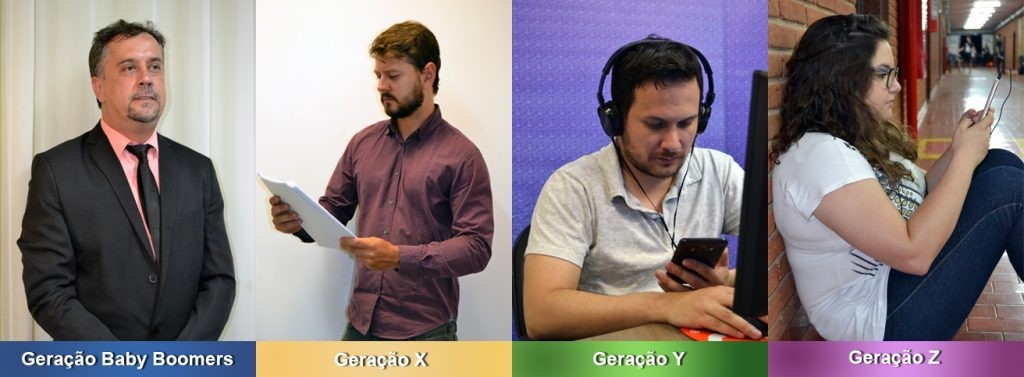
\includegraphics[width=0.6\textwidth]{fig02.png}
 \caption{Evolução das gerações, imagem extraída da tecnobiografia analisada.}
 \label{fig02}
 \source{Imagem da internet.\footnote{Disponível em: http://www.jornalismounaerp.com.br/blog/2017/12/13/baby-boomers-x-y-z-voce-sabe-qual-e-a-sua-geracao/}}
\end{figure}

De acordo com \textcite{jordao2016}, as gerações são definidas por indivíduos que sucederam seus pais. Durante muitas décadas as gerações surgiam a cada 25 anos, mas nos últimos 50 anos esse tempo vem diminuindo. Ainda segundo \textcite{jordao2016}, a Geração Baby Boomers (1940--1960) surgiu ao término da Segunda Guerra Mundial. O termo “Baby Boomer” pode ser traduzido para o português como “explosão de bebês”, que seria o momento em que os guerrilheiros voltam para suas casas e começam a criar suas famílias em um período de paz e prosperidade. A Geração X (1960--1980) seria constituída pelos nascidos durante a Guerra Fria em um tempo instável, na época da Ditadura militar no Brasil. As Gerações Y (1980--2000) e Geração Z (nascidos a partir dos anos 2000) seria formada pelos sujeitos da era das tecnologias digitais. A Geração Y acompanha de perto a popularização da internet e a Geração Z, em sua maioria, vive essa evolução tecnológica.

\textcite[p.~199]{gomes2016} faz algumas análises de metáforas encontradas em histórias de aprendizagem multimodais de estudantes de inglês. Nas imagens analisadas, os estudantes, ao narrarem suas experiências de aprendizagem, projetam-se metaforicamente “como seres que se engajam em caminhos, percursos e jornadas”, o que sugere a uma identidade metaforizada: o aprendiz é um viajante. 
Com a utilização das imagens (\Cref{fig02}), Clarice demonstra se representar enquanto usuária das novas tecnologias. Nessa conceitualização, é perceptível que ela está comprimindo e projetando vários anos de sua vida ao se identificar como uma pessoa pertencente às Gerações Baby Boomers, X, Y e Z, o que seria factualmente impossível.

Uma das imagens que \textcite{gomes2016} analisou se assemelha com a imagem utilizada por Clarice, como pode ser observado na \Cref{fig03}. 

\begin{figure}[htbp]
 \centering
 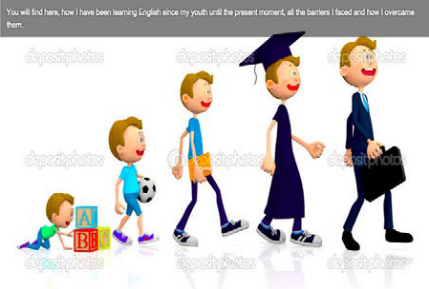
\includegraphics[width=0.6\textwidth]{fig03.png}
 \caption{Imagem analisada por \textcite{gomes2016}}
 \label{fig03}
 \source{\textcite{gomes2016}.}
\end{figure}

Na imagem analisada por \textcite[p.~206]{gomes2016}, há quatro indivíduos que são representações do narrador em diversos estágios de sua vida. Isso pode ser inferido por todos “terem a mesma aparência física (mesma cor de cabelo, mesma expressão facial)”. Na imagem apresentada por Clarice, as pessoas são diferentes em cor de pele, cabelo e gênero. Factualmente, Clarice não poderia ser essas quatro pessoas, ela está se metaforizando como uma pessoa que evoluiu tanto a ponto de ter passado por todas essas gerações. 

\subsubsection{Pequenas histórias}\label{sec-pequenas}
\textcite{barkuizen2014} trazem o conceito de pequenas histórias e descrevem como alguns pesquisadores trabalharam com essa temática. Eles citam a diferenciação de “grandes histórias” e “pequenas histórias”: as grandes retrospectivas extraídas de entrevistas e as narrativas efêmeras emergentes de situações cotidianas. 

Ainda segundo \textcite[p.~83]{barkuizen2014}, a “análise de posicionamentos” em pequenas histórias,

\begin{quote}
(\ldots) tem sido a principal estratégia de análise de dados na pesquisa de pequenas histórias, uma estratégia de análise de discurso que envolve identificação e interpretação das características interacionais através das quais os falantes identificam a si mesmo e os outros em termos de mútua compreensão e relações na interação e relacionamentos para contextos mais amplos do discurso (tradução nossa)\footnote{“has been the primary data analysis strategy in small story research, a discourse analysis strategy that involves identification and interpretation of the interactional features through which speakers identify self and others in terms of mutual relationships in interaction and relationships to wider contexts of discourse”.}.
\end{quote}

No caso da tecnobiografia de Clarice, dentro da macro história, em várias partes, ela “abre parênteses” e conta micro histórias, nas quais, além de se identificar dentro do contexto, menciona outros personagens em interações locais ou globais, como nos seguintes excertos:

\begin{quote}
(37) Ensinamos minha mãe a jogar e teve um dia que ela ficou em casa jogando o dia inteiro, pois estava sozinha e não sabia desligar o computador.

(38) A internet demorou a chegar na minha casa então eu ia para casa de amigos para dormir e esperava chegar meia-noite (era mais barato, visto que a internet era discada) para entrar nas salas de bate-papo e conhecer outras pessoas.  Neste tempo criei meu primeiro e-mail que era do BOL e conseguia falar com meus amigos de outras cidades. As cartas enormes que eu escrevia foram substituídas pelos e-mails.
\end{quote}

Os dois exemplos citados mostram fragmentos da memória de Clarice, pequenas histórias. No excerto (37), Clarice utiliza “ensinamos” (no plural), pois traz para sua narrativa outros sujeitos, que são seus irmãos, os quais procuravam envolver sua mãe nas tecnologias digitais. No excerto (38), Clarice menciona a interação com amigos (físicos e virtuais) em uma relação local e/ou global, para compartilhar conhecimentos e acaba descrevendo suas relações com as tecnologias digitais e novos conhecimentos como a criação e a própria utilização do e-mail ou encontro com outras pessoas nas salas de bate-papo. 

\subsubsection{Pequenas histórias de práticas de letramento}\label{sec-pequenas}
Uma tecnobiografia é um gênero frutífero para coleta ou análises de dados no que tange à prática social de leitura ou escrita (letramento) em plataformas digitais. \textcite{kleiman1995,soares1998} são algumas das pesquisadoras mais citadas quando o assunto é definir o conceito letramento e, ao fazerem um percurso histórico desse conceito, definem-no como leitura e escrita como prática social, que também será a perspectiva de análise nessa seção. 

\textcite{street2012} discorre sobre questões teóricas e práticas nos novos estudos do letramento (NSL) e sobre os conceitos “eventos de letramento” e “práticas de letramento”. Segundo o autor, as práticas de letramento devem ter o foco central em analisar situações e não simplesmente “descrever o que acontece nos contextos sociais em relação aos significados e aos usos do letramento” \cite[p.~70]{street2012}. Ainda segundo o autor, “eventos de letramento” é um conceito útil pois “capacita pesquisadores, e também participantes, a focalizar uma situação particular onde as coisas estão acontecendo” \cite[p.~75]{street2012} e exemplifica esses eventos como “verificar horários e tomar o ônibus, folear uma revista (\ldots)” \cite[p.~75]{street2012}. 

Nos excertos retirados da tecnobiografia de Clarice, podemos perceber eventos em que a leitura e escrita (letramento) são permeadas pelas tecnologias digitais:

\begin{quote}
(39) para entrar nas salas de bate-papo e conhecer outras pessoas.  Neste tempo criei meu primeiro e-mail que era do BOL e conseguia falar com meus amigos de outras cidades. As cartas enormes que eu escrevia foram substituídas pelos e-mails.

(40) Comecei a usar redes sociais como ICQ, MSN e Orkut. Com certeza o Orkut mudou a minha geração, reencontrei amigos de infância e fiz amizades nas comunidades com as pessoas que tinham os mesmos interesses que eu.

(41) Meus pais aprenderam a usar a internet para fazer compras, conversar com pessoas, marcar consultas e copiar/colar.
\end{quote}

Segundo \textcite[p.~76]{street2012}, “podemos fotografar eventos de letramento, mas não podemos fotografar práticas de letramento”. Nesse sentido, para entender as práticas de letramento, deve-se participar do contexto, conversar com as pessoas e ligar as experiências imediatas de leitura e escrita a outras coisas que as pessoas também façam.

\textcite[p.~76]{street2012} afirma ainda que “se observássemos um evento de letramento particular na condição de pessoa não-participante (\ldots) teríamos dificuldade de seguir o que estivesse acontecendo”. Assim sendo, para entender essas práticas de letramento, recorremos a Clarice para entender questões particulares dos excertos 39-41. Ao analisar os excertos 39 e 40, fica claro que houve uma ressignificação/transformação nas práticas de letramento da narradora e de sua família com o advento das tecnologias digitais. Por exemplo, a escrita de cartas que era mediada pelas tecnologias “caneta” e “papel” passa para a escrita de “e-mail”, por meio das teclas do computador e, em seguida, do touch screen do smartphone. 

\textcite{street2003}, ao se referir à relação local e global na ressignificação das práticas de letramento e ao impacto da era das, então, novas tecnologias, com a invenção da imprensa, surgimento de novas mídias, cita Giddens (1991), que pesquisa

\begin{quote}
(\ldots) de que maneira o telégrafo afetou a circulação em massa dos jornais e, mais tarde, o desenvolvimento da comunicação eletrônica. Todas essas mídias, sugere Giddens, alteraram a relação entre local e distante, assim como televisão, filmes e vídeos \cite[p. 2828, tradução nossa]{street2003}\footnote{“(\ldots) on the way the telegraph affected the mass circulation of newspapers and, latterly, the development of electronic communication. All of these media, Giddens suggests, altered the relationship between local and distant, as did television, films and videos”.}.
\end{quote}

Com o advento das novas tecnologias, na família de Clarice as práticas de letramentos vão se ressignificando, podendo ser percebidas na maneira que passam a utilizar a leitura e escrita, por exemplo, para conhecer outras comunidades e fazer novas amizades. Os pais dela agora também leem folhetos promocionais na internet e realizam compras sem sair de casa, marcam consulta pela internet, além de se engajarem em outras práticas de letramento nas tecnologias digitais. 

\section{Considerações finais}\label{sec-consideracoes}
Como mencionado neste artigo, as narrativas são produzidas por pessoas reais; portanto, o que falam ou escrevem traz significados de suas experiências dentro do contexto de sua narração. Segundo \textcite{clandinin2011}, devemos pensar a experiência (narrativa) além da “caixa preta”. Assim sendo, qualquer investigação é definida pelo que nomeiam de espaço tridimensional, que são: interação (pessoal e sociedade); continuidade (passado presente e futuro) combinado à situação (noção de lugar). Esse espaço tridimensional foi explorado na tecnobiografia analisada.

Na perspectiva da natureza dialógica do discurso \cite{bakhtin1981}, ao utilizarmos a linguagem em relação ao outro, somos, da mesma forma, influenciados pelo outro. Assim, a construção identitária acontece também de forma dialógica, na interação. De acordo com \textcite[p.~94]{moita2002},

\begin{quote}
[a]o mesmo tempo em que levamos em consideração a alteridade quando nos engajamos no discurso, também podemos alterar o outro e o outro pode nos modificar. Ou seja, ao mesmo tempo em que consideramos as identidades dos participantes discursivos, estamos também (re-)construindo as identidades deles nas práticas discursivas nas quais estamos envolvidos e eles estão (re-)construindo as nossas através do discurso.
\end{quote}

Dessa forma, nessa relação de alteridade, analisar a tecnobiografia de Clarice fez com que olhasse para minha trajetória em relação ao processo de aprendizagem com as tecnologias digitais. Clarice e eu nascemos na mesma década e, por sermos alunos do mesmo programa de pós-graduação, estamos ocupando um espaço em comum. Nossas semelhanças fizeram-me comparar nossas trajetórias, o que também ressaltou nossas diferenças. 

A primeira diferença é que Clarice nasce e cresce na região metropolitana de Belo Horizonte, Minas Gerais, e sou eu natural de uma comunidade do campo, no vale Jequitinhonha, localizada no interior de Minas, onde nasci, cresci e vivo até os dias atuais.  Percebi que Clarice teve o contato com as tecnologias digitais bem antes de mim. Ela entra na faculdade em 2003 e eu em 2015. Em 1997 ela teve seu primeiro computador; eu, em 2007, vi um computador pela primeira vez e, em 2009, consegui comprar o primeiro computador, utilizando o seguro de desemprego. 

Clarice relata que na universidade ganhou o primeiro celular. Ela não diz a data, mas foi entre 2003 e 2007, período em que ela estava na universidade. Eu tive o primeiro celular em 2015, que foi na mesma época em que chegou a telefonia celular em minha comunidade. Enquanto o Orkut muda a geração de Clarice, o Facebook e WhatsApp mudam a geração de minha comunidade.

\textcite{clandinin2011} afirmam que pesquisar sobre uma experiência é experienciá-la simultaneamente. E neste trabalho esse experienciar foi abordado por pelo menos duas perspectivas. Primeiramente, analisar a tecnobiografia de Clarice foi um processo de muita reflexão, pois faz parte da natureza da pesquisa narrativa “viver” a vida do outro. E a segunda perspectiva seria esse processo no qual o autor deste texto se identifica com a narradora e encontra semelhanças e diferenças que contribuíram para sua construção identitária. 

Por meio dessa análise narrativa, pude perceber a evolução de Clarice e até pensar nessa distância (temporal) e de acessibilidade entre campo e cidade ao comparar nossas trajetórias. Através dessa comparação, percebe-se o papel da pesquisa narrativa na experiência humana ao ponto de fazer com que quem escreve reflita sobre sua vida, e quem lê reflita sobre a vida do outro e sua própria vida. Ou seja, o processo de narrar e analisar a narrativa do outro é um processo formativo.

\printbibliography\label{sec-bib}
% if the text is not in Portuguese, it might be necessary to use the code below instead to print the correct ABNT abbreviations [s.n.], [s.l.] 
%\begin{portuguese}
%\printbibliography[title={Bibliography}]
%\end{portuguese}

\end{document}
